En este apartado se presentara el diseño del software derivado de la especificación, este diseño busca representar la estructura que tendrá que tener el software y los patrones que se aplicaran, todo con el objetivo de mejorar la escalabilidad, portabilidad y reusabilidad.
Con este objetivo se desplegara el diagrama de modelo conceptual de datos (ver apartado \ref{sec:modelo_conceptual_datos}) concretando la estructura con la que se tendrá que desarrollar el sistema y se explicara la arquitectura que se usara para llevarlo a cabo.


Para poder entender los diagramas de diseño primero introduciremos los patrones usados en el proyecto, gran parte de estos patrones están extraídos del libro Design patterns\cite{vlissides1995design}.

\subsection{Patrones de arquitectónicos}
\subsubsection{Modelo vista controlador}
\label{sec:mvc}
Para el desarrollo del proyecto se usara el framework de desarrollo Django, este framework esta diseñado para seguir la arquitectura modelo , vista, controlador. Con la puntualidad que se ha modificado la nomenclatura a modelo, vista, template.\\
\begin{figure}[ht!]
\center
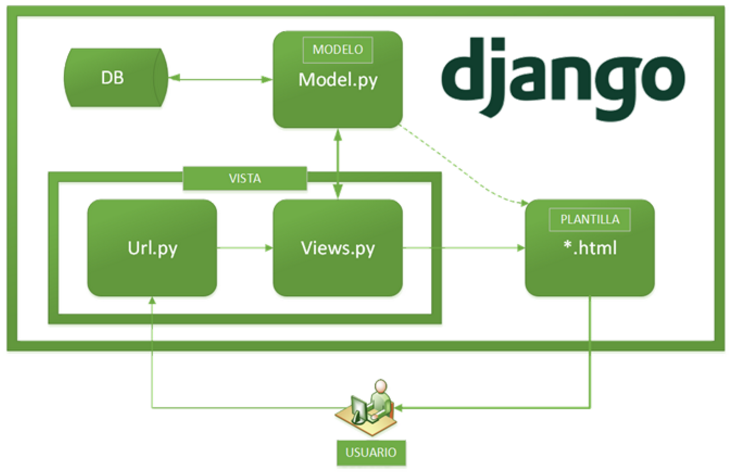
\includegraphics[scale=0.6]{diagramas/django_architecture.png}
\caption{Arquitectura propuesta por el framework Django}
\label{fig:django}
\end{figure}
\\
Los modelos son los encargado de contener las clases que representan nuestro modelo de datos, en las vistas se encuentra la lógica de la aplicación y en las plantillas se renderizá el resultados para presentarlo al usuario.
Para este proyecto se ha usado otro framework que trabaja sobre Django, Django API rest framework, este nos proporciona herramientas para llevar a cabo APIs rest con Django, una de estas herramientas son los seralizadores, encargados de transformar nuestras respuestas a json o XML, de tal forma que nuestra arquitectura finalmente quedaría de la siguiente forma.
\\
\begin{figure}[ht!]
\center
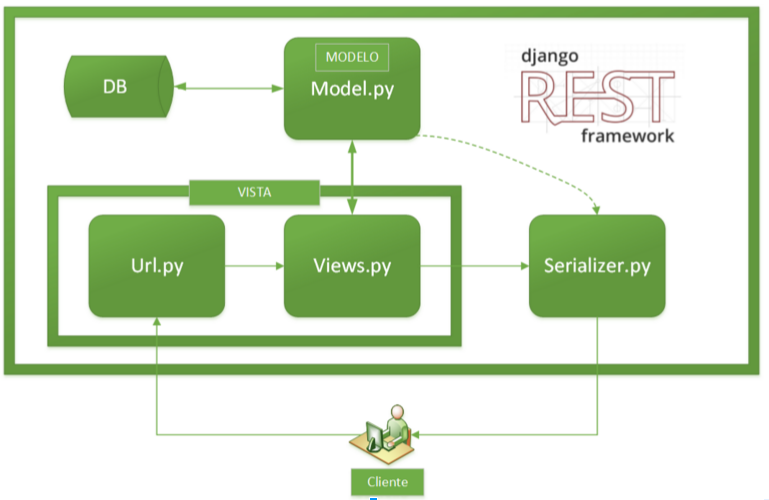
\includegraphics[scale=0.7]{diagramas/rest_fram_architect_adap.png}
\caption{Arquitectura propuesta por Django Rest Framework}
\label{fig:rest_framework}
\end{figure}
\\
El objetivo final de este patrón es separar la representación interna de la información de la manera en que la información es presentada o aceptada. De esta forma, en el proyecto, la persistencia solo es tratada en los modelos, la lógica del sistema en las vistas y la presentación en los serializadores.

\subsubsection{Message Broker}
\label{sec:message_broker}
Es un patrón usado para la validación de mensajes, transformación y enrutamiento. El ``message broker'' hace de mediador entre aplicaciones  permitiendo el paso de mensajes entre ellas sin necesidad de tener en cuenta el estado del sistema emisor o receptor.

En este proyecto se ha usará Celery y RabitMQ para desplegar este patrón arquitectónico. Cerlery se encarga de encolar los mensajes y configura nuestros workers que consumirán del ```message broker'' en este caso RabitMQ.

Con este patrón arquitectónico se se basa en el patrón de mensajes  ``publish–subscribe'', en el apartado destinado a patrones de mensajes se explicara en detalle este patrón.

La figura \ref{fig:celery_architecture} podemos ver un diagrama de la arquitectura de este patrón con las tecnologías que se han decidido usar.
\begin{figure}[ht!]
\center
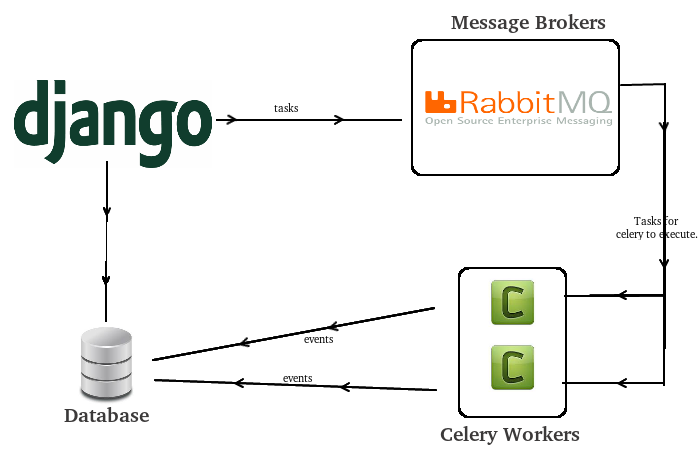
\includegraphics[scale=0.5]{django_celery_architecture.png}
\caption{Arquitectura para usar message broker}
\label{fig:celery_architecture}
\end{figure}
 \newpage
 Se ha decidido usar este esté patrón arquitectónico para hacer que ciertas tareas muy pesadas del sistema se hagan de forma distribuida, concurrente y asíncrona, esto hará que el usuario si requiere una de las tareas que siguen este patrón pueda recibir un mensaje de aceptación y ser notificado cuando la tarea termine.
 Las tareas son la subida de archivos Gedcom y la búsqueda de usuarios similares.

\newpage
\subsubsection{REST}
REST es el acrónimo de a Transferencia de Estado Representacional (Representational State Transfer), es un estilo de arquitectura para sistemas de hipermedia(i.e. término con el que se designa al conjunto de métodos o procedimientos para escribir, diseñar o componer contenidos) distribuidos.
Las arquitecturas REST usan el protocolo HTTP para dará acceso a los recursos del sistema. Los fundamentos clave de REST son:
\begin{description}
\item[Protocolo cliente/servidor sin estado]: Cada mensaje HTTP contiene toda la información necesaria para comprender la petición. Como resultado, ni el cliente ni el servidor necesitan recordar ningún estado de las comunicaciones entre mensajes. 
\item[Operaciones bien definidas]: HTTP en sí define un conjunto pequeño de operaciones, las más importantes son POST, GET, PUT y DELETE. Con frecuencia estas operaciones se equiparan a las operaciones CRUD en bases de datos.
\item[Sintaxis universal]: En un sistema REST cada recurso es accesible únicamente a través de su URI.
\item[Uso de hipermedios]: Las respuestas llevan referencias a los recursos con los que esta relacionado el recurso consultado, permitiendo navegar entre ellos. 
\end{description}
Se ha optado por el uso de este patrón ya que permite a nuestro sistema ser utilizado desde cualquier plataforma (aplicaciones móviles, \textit{front-ends} web), dado que toda la comunicación REST se realiza por protocolo HTTP.

\subsection{Patrones de mensajería}
\subsubsection{\textit{Publish–subscribe}}
\label{sec:pub-sub}
El patrón \textit{publish-subscribe} consiste en plantear un sistema de envió de mensajes entre dos entidades, una encargada de enviar los mensajes, llamada \textit{publisher} y otra encargada de tratarlos, llamada \textit{subscriber}. El patrón establece que tanto el \textit{publisher} como el \textit{subscriber} tienen que funcionar de manera independiente, es decir que no necesiten saber de la existencia de estos.
Esto se consigue mediante una cola de mensajes, en este proyecto sera RabitMQ como se ha explicado en el apartado en el que se explica el patrón \textit{message broker}\ref{sec:message_broker}.
Las ventajas de este patrón son:
\begin{description}
	\item Mayor escalabilidad de la infraestructura. Esta escalabilidad la conseguiríamos creando nuevos \textit{subscribers} que escuchen a la cola de tareas.
	\item Reducción del acoplamiento, dado que tanto el \textit{publisher} como el \textit{subscriber} pueden funcionar de forma independiente uno del otro.
\end{description}

\subsection{Patrones Estructurales}
\subsubsection{Mixins}
Un mixin es una clase que ofrece funcionalidades y puede ser heredada por una subclase, estas clases no están pensadas para funcionar de forma autónoma. Se puede entender como una inyección de código.
Este patrón refuerza el principio de inversión de dependencias (i.e. una forma de reducir el grado de interdependencia entre los módulos).
Este patrón estructural es el que usa Django rest framework para facilitar la creación de vistas. El framework nos proporciona varios \textit{mixins} que contienen las llamadas a los serliazadores necesarias para efectuar las operaciones CRUD sobre un modelo.

\subsection{Protocolos}
Como ya se ha comentado en los apartados anteriores la API a desarrollar sera REST, en consecuencia al autenticar y autorizar de los usuarios que hagan uso de nuestra API se tendrá que hacer de una forma que el sistema no necesite conservar el estado. Para ello se usara oAuth 2, un protocolo que permitirá autenticar y autorizar a nuestros usuarios en el sistema.

\subsubsection{OAuth 2}
\label{sec:oauth2}
La funcionalidad básica de oAtuh 2 es permitir a terceros autenticar usuarios contra un sistema, mediante el uso de tokens. Para ello se vale de diferentes mecanismos. para este proyecto se usara el mecanismo \textit{password based}, que no permite aislar el control de las credenciales de usuario a las clientes que usan nuestra API pero por contrapartida su mecanismo es más simple.
Primero definiremos la nomenclatura que se usara.
\begin{description}
\item[User]: Es el usuario final que almacenara los datos en nuestra API.
\item[Client]: Es una aplicación de terceros que da servició a los usuarios haciendo de interfaz entre la API y el usuario.
\item[Provider]: API contra la que los clientes se pueden autenticar mediante oAtuh.
\item[Client secret y client id]: Estos dos elementos identifican a un cliente, son las credenciales que este usa para conseguir los tokens que permiten a los usuarios validarse.
\item[Resource]: Un \textit{resource} es un recurso almacenado por un \textit{user} que nuestra API almacena.
\item[Acces token]: Un \textit{acces token} es el token que una vez obtenido por el cliente le permite validar al usuario que lo esta usando contra nuestra API. Para mejorar la seguridad, los tokens tendrán un tiempo de vida, con lo que se tendrán que ir renovando.
\end{description}
A continuación se adjunta un diagrama genérico de los pasos que tiene que seguir un cliente, para adquirir un recurso usando las credenciales de un usuario.

\begin{figure}[ht!]
\center
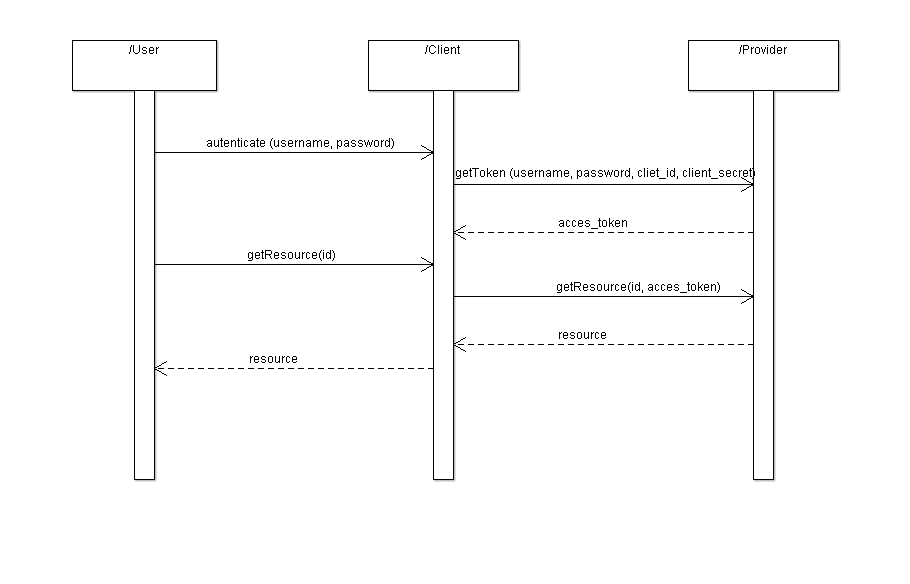
\includegraphics[scale=0.55]{diagramas/oatuh.png}
\caption{Diagrama para de autenticación con OAuth, password based}
\label{fig:auth_sequence1}
\end{figure}

El siguiente diagrama representa el flujo para pedir un token de renovación.
\begin{figure}[ht!]
\center
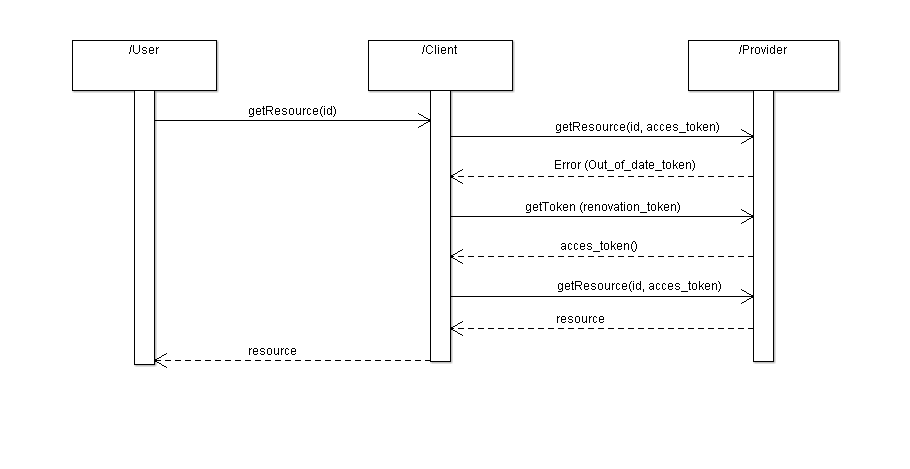
\includegraphics[scale=0.55]{diagramas/renovation_token.png}
\caption{Diagrama para renovar acces token con oAuth}
\label{fig:auth_sequence2}
\end{figure}
\newpage

Como podemos ver en la figura \ref{fig:auth_sequence1} la interacción empieza con el intento de autentificación de un usuario mediante una aplicación. Seguidamente la aplicación se identifica contra el \textit{provider} proporcionando sus credenciales y las del usuario. Como resultado el \textit{privider} retorna un \textit{acces token} que permitirá autentificar al usuario con los permisos que este disponga. Con este \textit{acces token} el cliente podrá pedir recursos al \textit{provider} y este podrá usar las credenciales del token para autentificar al usuario en cada petición y saber sus permisos.

En la figura \ref{fig:auth_sequence2} vemos como se realiza la renovación de un token una vez el cliente se da cuenta que este a caducado. La secuencia empieza con una llamada del cliente para conseguir un recurso, a lo que el \textit{provider} responde con un mensaje de error notificando que el token ya no es valido. Seguidamente el cliente hace una llamada a la uri usada para conseguir el token, con el \textit{renovation token} y el provider retorna un nuevo token.

El funcionamiento de todo el protocolo esta definido en el RFC 6750 titulado The OAuth 2.0 Authorization Framework\cite{oauth2rfc}.

En la fase de implementación se explicara con que endpoints concretos se usaran estas funcionalidades y que parámetros se tendrán que proporcionar.

\subsection{Diseño del modelo de datos}
\label{sec:diseno_modelo_datos}
El sistema a desarrollar es una API rest-ful que permita la interacción de aplicaciones de terceros sobre nuestros datos, con ese objetivo nuestro modelo ha de constar de mecanismos para que estos terceros se autentiquen contra nuestro sistema. Para ello se implementara un sistema para autenticar y autorización basado en oAuth 2.0 como se ha explicado en el apartado \ref{sec:oauth2} , el diagrama especificado a continuación amplia el del modelo conceptual de datos que podemos ver en la figura \ref{fig:data_model} añadiendo todas las clases necesarias para su futura implementación con los patrones y protocolos explicados en los apartados anteriores.

\begin{figure}[ht!]
\center
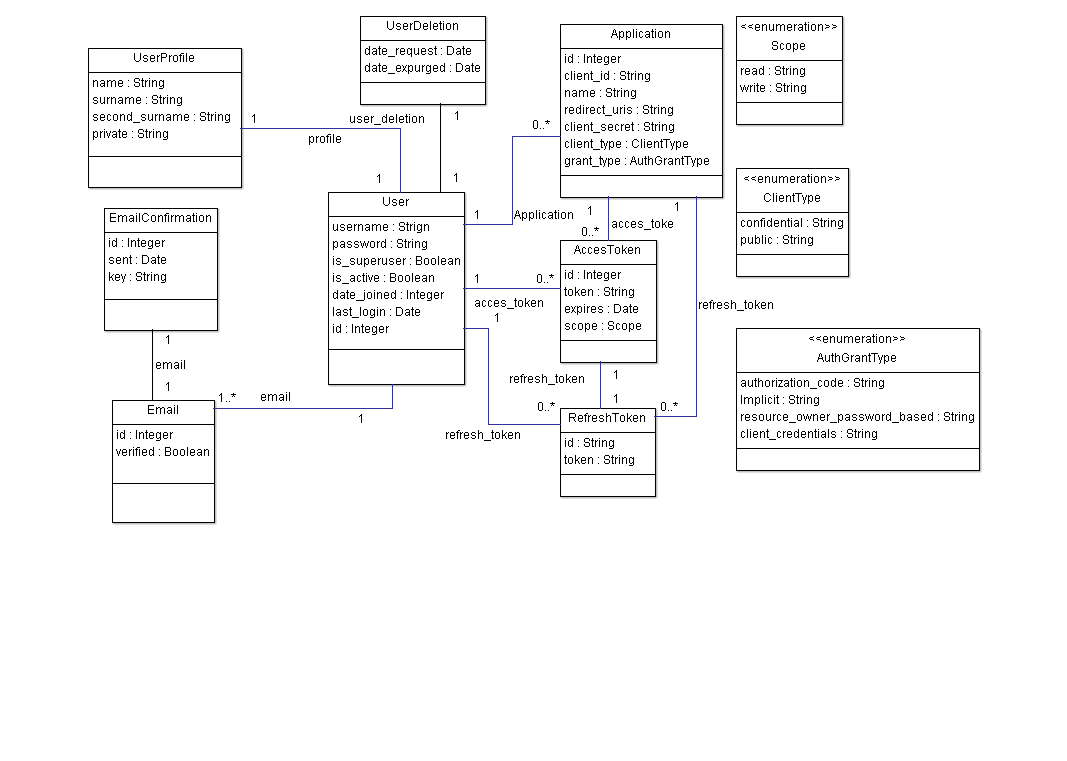
\includegraphics[scale=0.45]{diagramas/sqldiagram.png}
\caption{Diagrama modelo de datos relacional}
\label{fig:sqldiagram}
\end{figure}
\newpage
Se ha decidido que la gestión de usuarios se hará usado modelo relacional, esta decisión se a tomado teniendo en cuenta que nuestro sistema no realiza consultas donde se tenga que recorrer el modelo, por lo que no tiene sentido usar una base de datos orientada a grafos, en lo que se refiere a al gestión de usuarios. De esta forma también se puede aprovechar las librerías que proporciona Django para la gestión de usuarios, que usan el modelo relacional.

A continuación se explican las clases definidas en el diagrama:
\begin{description}
	\item[User]: Representa un usuario del sistema, sus atributos son los datos esenciales para que este pueda hacer uso del sistema.
	\item[UserProfile]: Representa los datos personales de un usuario.
	\item[Email]: Representa un correo electrónico que esta asociado a un usuario.
	\item[EmailConfirmation]: Contiene los datos referentes a la validación de un correo electrónico de un usuario. La key es la clave que el usuario tiene que usar para validar el correo y sent la fecha en la que se ha enviado el correo pidiendo la validación.
	\item[UserDeletion]: Contiene las peticiones de borrado de cuenta de los usuarios, date\_request indica la fecha en la que se ha realizado la petición de eliminación y date\_expurged la fecha en que la cuenta debe ser borrada definitivamente del sistema.
	\item[Application]: Esta clase se refiere a los clientes que dan de alta los usuarios. Estos clientes son las aplicaciones de terceros que están dadas de alta para usar nuestro sistema. Se incluyen todos los atributos necesarios establecidos por el RFC que describe oAuth \cite{oauth2rfc} para describir un cliente. A pesar que solo se usaran los mencionados en el apartado de diseño \ref{sec:oauth2}.
	\item[AccesToken]: Contiene los AccesToken que ha solicitado un cliente. Contiene todos los atributos especificados en el RFC que describe oAuth2, de la misma forma que en \textit{Aplication}.
	\item{RefreshToken}: Esta clase contiene el \textit{refresh token} necesario para renovar un \textit{acces token} que ya ha expirado, tal como se explica en el apartado \ref{sec:oauth2}.
\end{description}
\newpage
A continuación, en la figura \ref{fig:graphdiagram} se encuentra el diagrama de diseño del árbol genealógico:

\begin{figure}[ht!]
\center
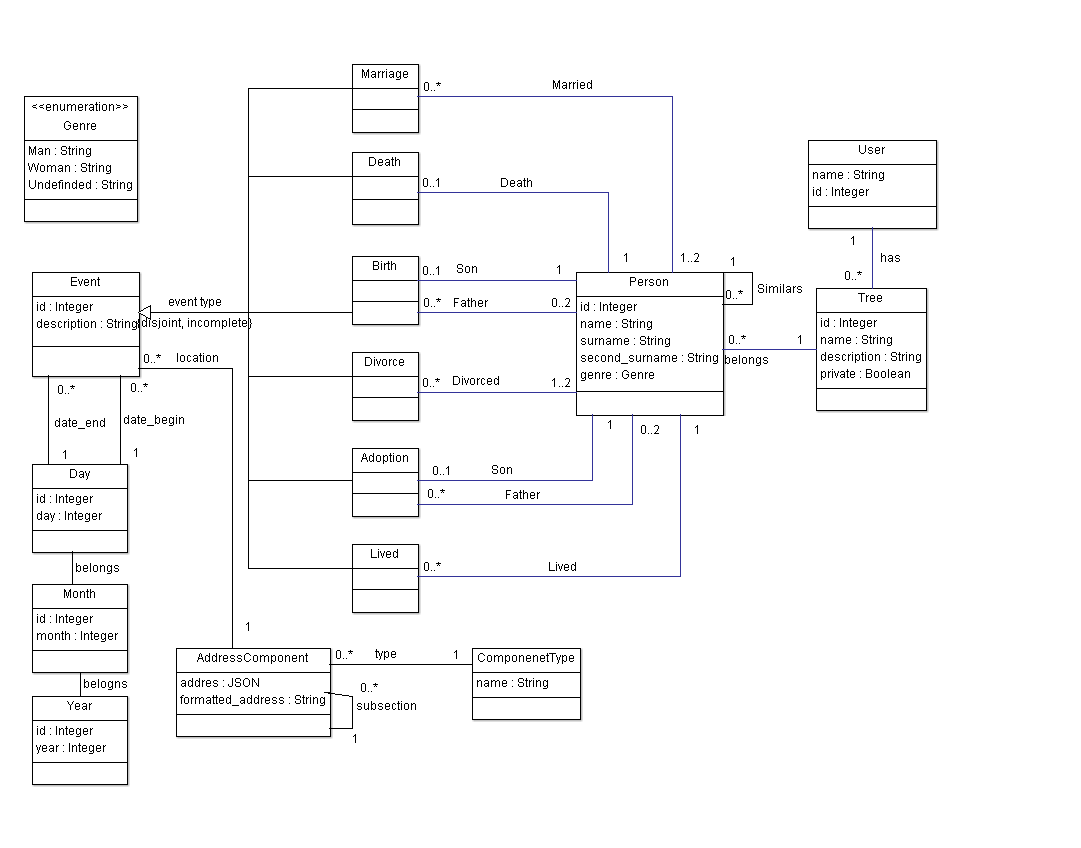
\includegraphics[scale=0.45]{diagramas/graphdiagram.png}
\caption{Diagrama modelo de datos orientado a grafos}
\label{fig:graphdiagram}
\end{figure}

Esta parte del modelo de datos se implementara usando un modelo orientado a grafos, ya que es sobre los datos que nuestro sistema tendrá que realizar gran parte de consultas que requieren recorrer el domino. El diseño esta hecho de tal forma que se pueda aprovechar la adyacencia libre de indice explicada en el apartado \ref{sec:bdog}.
 
La clase \textit{User}, sera un nodo que compartirá el id con el de la clase \textit{User} de la base de datos relacional, para poderse referenciar de forma cruzada.\\
En las siguientes selecciones se explica como se ha diseñado más concertadamente las fechas y las localizaciones en el modelo orientado a grafos y los beneficios de este diseño, las otras clases siguen la misma definición que las del modelo conceptual definido en la sección \ref{sec:smodelo_conceptual_datos}.
\newpage
\subsubsection{Arboles temporales.}
Con el objetivo de aprovechar la adyacencia libre de indice los las DBOG se implementara una estructura arbórea donde se representaran las fechas, esta estructura se propone en el libro GrapDB \ref{fig:grdb}, esto nos permitirá gran rapidez a la hora de consultar todos los eventos que hayan sucedido en un año, mes o día. Podemos ver un ejemplo de su estrucutra en la figura \ref{fig:timeline}

\begin{figure}[ht!]
\center
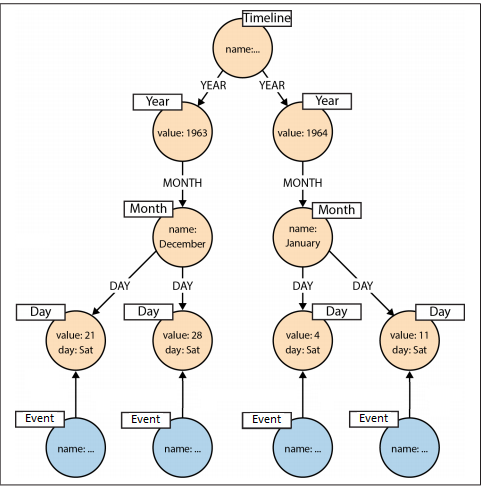
\includegraphics[scale=0.7]{timeline_tree.PNG}
\caption{Ejemplo de un \textit{timeline} tree}
\label{fig:timeline}
\end{figure}

En esta estructura llamada \textit{Timeline tree} \ref{fig:timeline} cada año tiene su propio conjunto de meses y cada mes tiene su propio conjunto de días. Para mantener la estructura solo tenemos que añadir nodos cuando estos sean necesarios.

Los nodos Year, Month y Day representan las clases con el mismo nombre del diagrama de la figura \ref{fig:graphdiagram}.
\newpage
\subsubsection{Geocomponentes}
Aplicando la misma lógica que para las fechas también se creara una estructura arbórea para las localizaciones. La peculiaridad de esta estructura es que cualquier elemento del árbol podrá tener una relación con el evento, en caso que no se pueda concretar la localización con más detalle. Y de la misma forma que en el \textit{timeline tree} los nodos serán únicos, por lo que solo se tendran que crear en el caso que no existan ya en la base de datos. Podemos ver un ejemplo de esta estructura en la figura \ref{fig:location_line}.

\begin{figure}[ht!]
\center
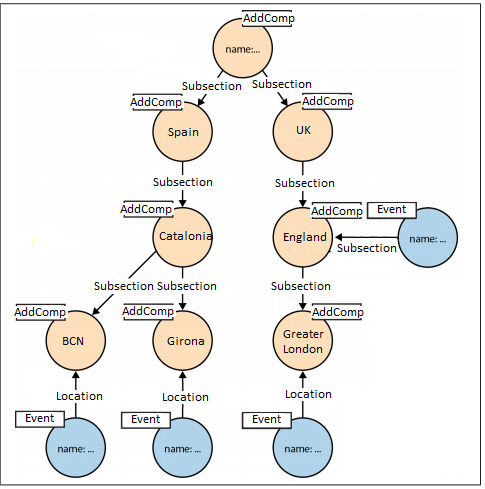
\includegraphics[scale=0.7]{geocomponent_tree.PNG}
\caption{Ejemplo de un árbol de geocomponentes}
\label{fig:location_line}
\end{figure}

\newpage

\subsection{Diseño de la capa de dominio}
Se harán dos diagramas con el fin de mejorar la comprensibilidad de estos, uno correspondiente al \textit{publisher} y otro al \textit{subscriber}, siguiendo la nomenclatura definida en la explicación del patrón \textit{publish-subscriber} \ref{sec:pub-sub}.

A continuación explicaremos el diagrama del \textit{publisher}, que podemos ver en la figura \ref{fig:domino}. Este diagrama esta simplificado y no contiene las clases referentes a los eventos, si bien siguen la misma estructura que las clases referentes a las personas y arboles.

Podemos diferenciar 3 componentes principales siguiendo la adaptación del patrón MVC explicado en la sección \ref{sec:mvc}, estos componentes son: 
\begin{description}
	\item[\textit{Models}]: Estos contienen los atributos especificados en el apartado \ref{sec:smodelo_conceptual_datos}, más concretamente en la figura \ref{fig:graphdiagram}. Y todas las operaciones necesarias para tratar estos datos. Dado que Neo4j no permite definir restricciones de integridad en el SGBD se ha creado una clase \textit{restriction}, donde se implementan todas y son llamadas desde el modelo, ejecutándose antes de realizar las operaciones que necesiten comprobar alguna restricción. En el diagrama salen representados como las clases \textit{Person} y \textit{Tree}
	
	\item[\textit{Views}]: Se han implementado usando los \textit{mixins} que proporciona API rest framework, estas clases añaden las operaciones equivalentes a las operaciones CRUD de nuestra base de datos llamando a los seralizadores que definimos en nuestras vistas, en este caso \textit{TreeViewSet} y \textit{PersonViewSet}. Por otro lado la clase APIView nos proporciona herramientas para tratar las request, que contienen la información de la petición a tratar. Por ultimo Response es una clase de Django nos da las opreaciónes que nos permiten enviar una respuesta a la \textit{request} solicitada.
	
	\item[\textit{Serializers}]: Estas clases se encargan de serializar y desserializar la información que llega en la \textit{request}. Para implementar los serializadores se ha usado la clase BaseSerializer de API rest framework, esta clase nos proporciona las funciones que las clases \textit{mixin} de las vistas usaran para realizar sus operaciones, el atributo \textit{many} nos permite serializar y deserializar conjuntos de datos en caso que este sea \textit{True}. Para poder usar esta clase tenemos que implementar los métodos definidos en nuestros serializadores, \textit{TreeSerializer} y \textit{PersonSerializer}. to\_internal\_value se encarga de transformar los datos que llegan de la \textit{request} en forma de string los tipos de datos que se usen en el sistema, estos datos se guardaran en el atributo valid\_data, to\_representation recibe un objeto de nuestra base de datos y lo serializa a un JSON con los datos que retorna a una petición, por ultimo \textit{create} y \textit{update} realizan dichas operaciones con la información que to\_internal\_value a convertido a tipos de datos que usa nuestro sistema.
\end{description}

A continuación se explican las otras clases y se explica su función.
\begin{description}
\item[permissions]: Esta clase es un ejemplo de un permiso al que esta restringida una \textit{view}. Antes de ejecutar ninguna operación, las \textit{views} comprueban que todos los permisos se cumplan. Las \textit{views} del sistema usan los siguientes permisos:
\begin{itemize}
	\item IsAuthenticated: Comprueba que el usuario que realiza la \textit{request} esta autenticado
	\item TokenHasReadWriteScope: Comprueba que el usuario que realiza la \textit{request} tenga permisos de lectura y escritura sobre los recursos accedidos.
\end{itemize}
\item[router]: Esta clase es la encargada de enturar las peticiones según el \textit{endpoint} por el que han llegado a las \textit{views} correspondientes
\item[celery]: Esta clase es la encargada de enviar las tareas al \textit{message broker}, tal y como se explica en el apartado \ref{sec:message_broker}. Para enviar la tarea de cargar un gedcom, lo que hace es serializar la función que realiza esta tarea y la envía mediante la función async al \textit{message broker}.
\end{description}

\begin{figure}[ht!]
\center
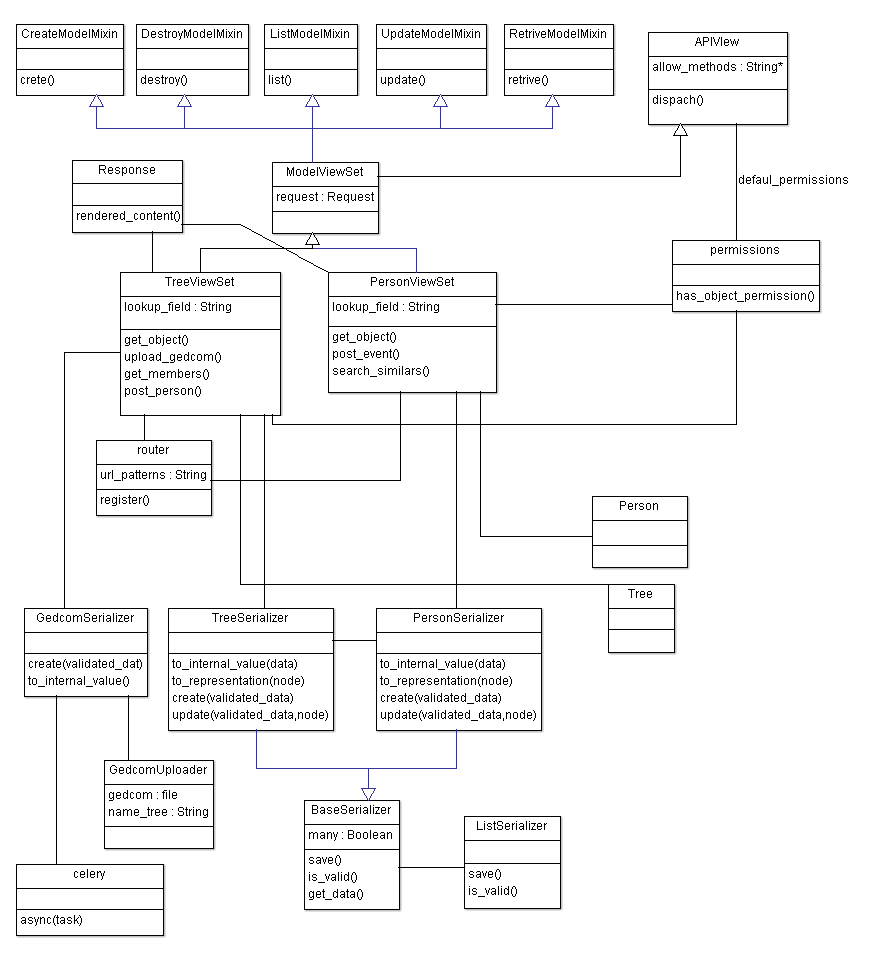
\includegraphics[scale=0.4]{diagramas/dominio2.png}
\caption{Diagrama de la capa de domino}
\label{fig:domino}
\end{figure}

Ahora se explicara el diagrama del \textit{subscriber} encargado de tratar con las tareas de cargar un GEDCOM.
El diagrama lo podemos ver en la figura \ref{fig:domino2} .

\begin{figure}[ht!]
	\center
	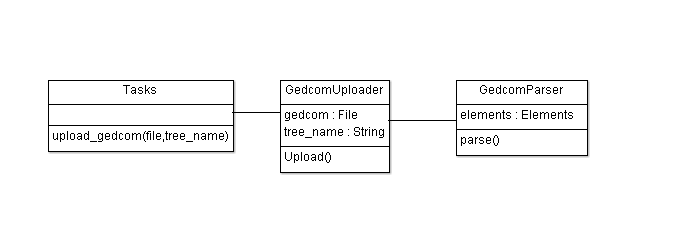
\includegraphics[scale=0.4]{diagramas/dominio3.png}
	\caption{Diagrama de la capa de domino}
	\label{fig:domino2}
\end{figure}

\textbf{pendiente}
\newpage
\subsection{Diseño del modelo de comportamiento}
En este apartado se incluyen los diagramas del modelo de comportamiento para las funcionalidades del sistema. Para la comunicación entre los modelos vistas y serializadores se hará un diagrama que generalice el funcionamiento. Para las operaciones más concretas se añadirá un diagrama para cada una.

Como ejemplo se usara la obtención de una persona.

\begin{figure}[ht!]
\center
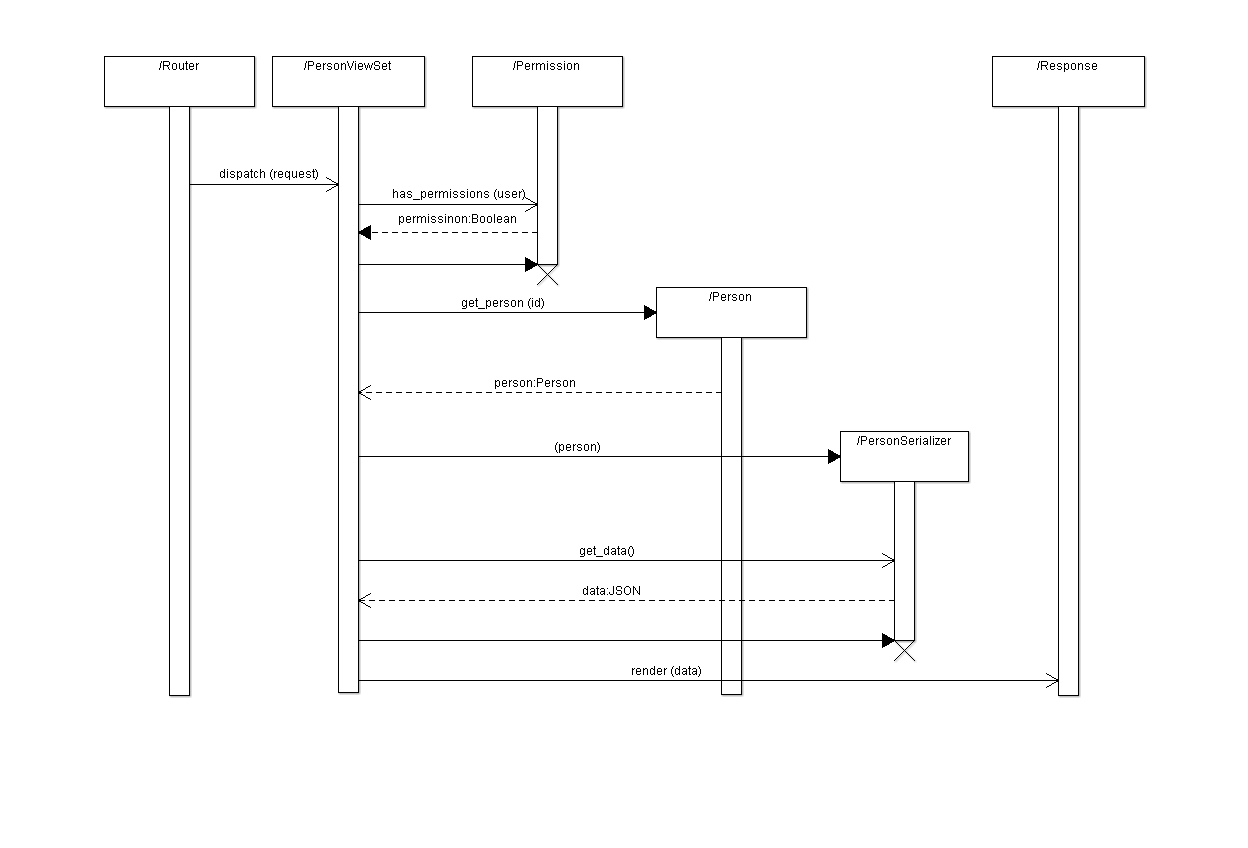
\includegraphics[scale=0.4]{diagramas/getPerson.png}
\caption{Diagrama de secuencia para obtener una persona}
\label{fig:sequence_diagram_get_person}
\end{figure}

Aquí se adjunta un diagrama de una operación más compleja, pero que lógicamente sigue la misma lógica que la anterior.
\begin{figure}[ht!]
\center
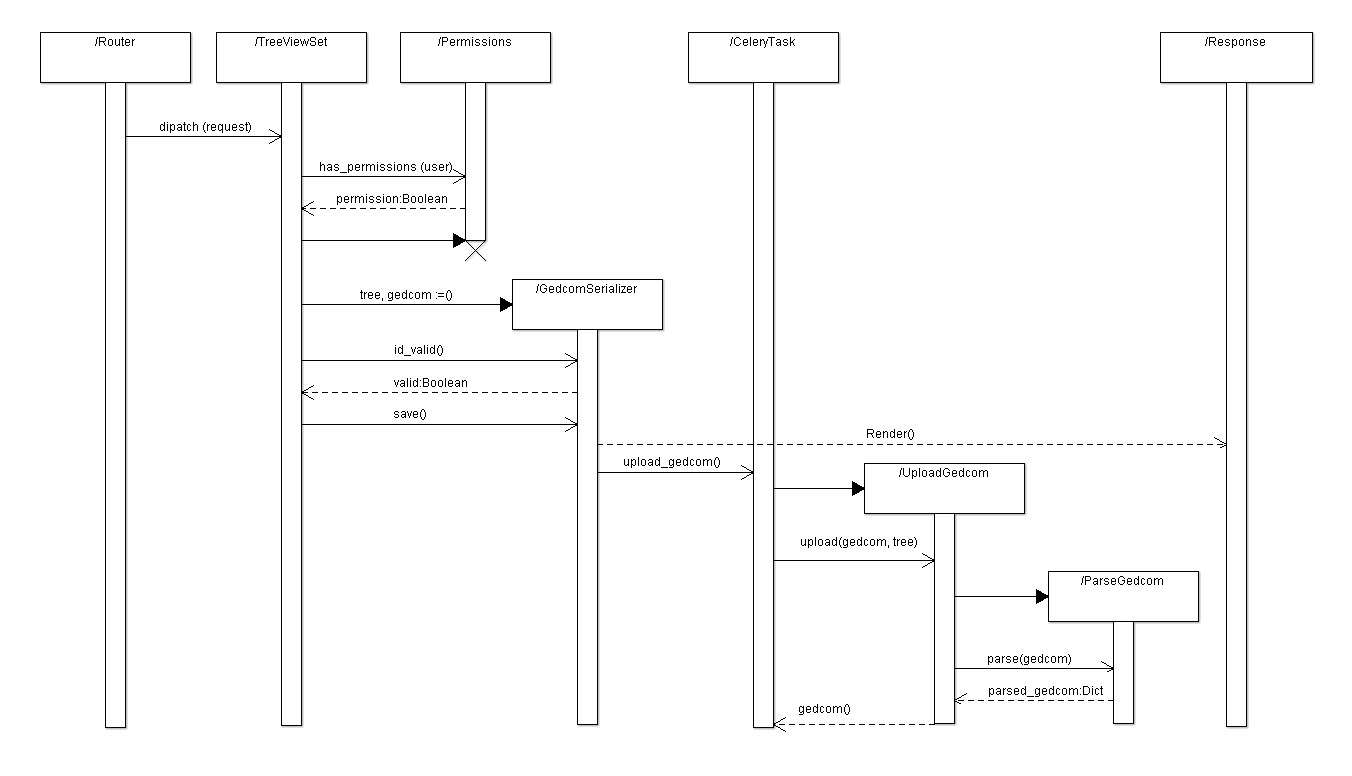
\includegraphics[scale=0.3]{diagramas/upload_gedcom.png}
\caption{Diagrama de secuencia para subir un archivo GEDCOM}
\label{fig:sequence_diagram_GEDCOM}
\end{figure}